\renewcommand{\thislecture}{9 }

%
% Cover page
%

\title[Neutrino Physics / Lecture \thislecture]
{
  {\huge \color{yellow} Neutrino Physics - Lecture \thislecture} \\
  {\it Deep Inelastic Scattering and Hadronization}\\
}

\author[C.Andreopoulos] {
  Professor Costas Andreopoulos\inst{1,2}
}
\institute[Liverpool/STFC-RAL] {
   \inst{1} University of Liverpool,
   \inst{2} STFC Rutherford Appleton Laboratory\\
   \vspace{0.5cm}
   {\it {\color{magenta} A post-graduate student lecture course}}\\
   \vspace{0.2cm}
}
\date{\today}

\titlegraphic{
  
\includegraphics[height=25px]{./images/logo/liverpool.png}
  \hspace{3px}
  
\includegraphics[height=30px]{./images/logo/ral.png}
}

	



\begin{frame}[plain]
  \titlepage
\end{frame}

%
% Outline
%

\begin{frame}{Outline for Lecture \thislecture}

\begin{itemize}
\item Brief description of the GENIE hadronization model.
\item Data/MC comparisons.
\item Systematic handles.
\item Thoughts for hadronization systematics in VALOR.
\end{itemize}

\end{frame}


%
%
%


\begin{frame}{Basic picture}

\end{frame}




\begin{frame}{Kinematics}

\begin{columns}[T]
  \begin{column}{0.50\textwidth}
  {\small
  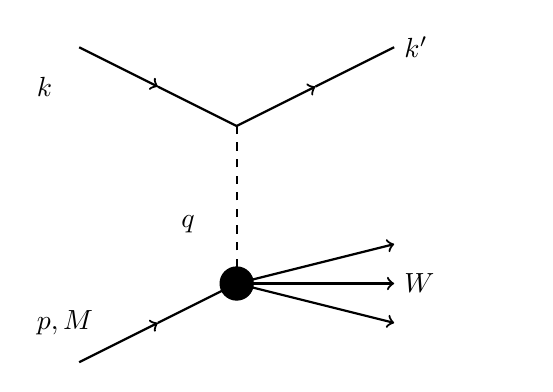
\begin{tikzpicture}
  \draw[solid,thick,black,->] (1,12.0) -- (2,11.5) node[left, text width=4em]{$k$};
  \draw[solid,thick,black,- ] (2,11.5) -- (3,11.0);
  \draw[solid,thick,black,->] (3,11.0) -- (4,11.5);
  \draw[solid,thick,black,- ] (4,11.5) -- (5,12.0) node[right, text width=4em]{$k^{\prime}$};
  \filldraw (3,9) circle (6pt);
  \draw[dashed,thick,black,- ] (3,9.0) -- (3,11.0) node[below, midway, text width=4em]{$q$};
  \draw[solid,thick,black,->]  (1,8.0) -- (2, 8.5) node[left, text width=4em]{$p,M$};
  \draw[solid,thick,black,- ]  (2,8.5) -- (3, 9.0);
  \draw[solid,thick,black,->]  (3,9.0) -- (5, 9.5);
  \draw[solid,thick,black,->]  (3,9.0) -- (5, 9.0) node[right, text width=4em]{$W$};
  \draw[solid,thick,black,->]  (3,9.0) -- (5, 8.5);
  \end{tikzpicture} 
  }
  \end{column}
  \begin{column}{0.50\textwidth}
  {\small
    $\displaystyle \nu = \frac{q \cdot p}{M} = E - E^{\prime}$\\
    $\displaystyle Q^{2} = -q^{2} = 2(E \cdot E^{\prime} - \vec{k} \cdot \vec{k^{\prime}}) \approx 4 E E^{\prime} sin^{2}(\theta/2)$\\
    $\displaystyle x = \frac{Q^{2}}{2M\nu}$\\
    $\displaystyle y = \frac{q \cdot p}{k \cdot p} = \frac{\nu}{E}$\\
    $\displaystyle W^{2} = (p+q)^{2} = M^{2} + 2M\nu - Q^{2}$\\
  }
  \end{column}
\end{columns}

\end{frame}




\begin{frame}{Inclusive cross-section}

\begin{equation*}
 d\sigma \propto L_{\mu\nu} W^{\mu\nu}
\end{equation*}

\begin{equation*}
 L_{\mu\nu} = k_{\mu} k_{\nu}^{\prime} + k_{\mu}^{\prime} k_{\nu} - g_{\mu\nu} k \cdot k^{\prime} - i {\epsilon}_{\mu\nu\rho\sigma} k^{\rho} k^{\prime \sigma}
\end{equation*}

\begin{equation*}
 W^{\mu\nu} = -g^{\mu\nu} {\color{red}W_{1}} 
              + \frac{p^{\mu}p^{\nu}}{M^{2}} {\color{red}W_{2}} 
              - i \frac{{\epsilon}^{\mu\nu\rho\sigma}p_{\rho}p_{\sigma}}{2M^{2}} {\color{red}W_{3}} 
              + \frac{q^{\mu}q^{\nu}}{M^{2}} {\color{red}W_{4}} 
\end{equation*}
\begin{equation}
              + \frac{p^{\mu}q^{\nu}+q^{\mu}p^{\nu}}{2M^{2}} {\color{red}W_{5}} 
              + i \frac{p^{\mu}q^{\nu}-q^{\mu}p^{\nu}}{2M^{2}} {\color{red}W_{6}} 
\end{equation}

\end{frame}


\begin{frame}{Structure functions}

{\scriptsize
\begin{equation*}
 W^{\mu\nu} = -g^{\mu\nu} {\color{red}W_{1}} 
              + \frac{p^{\mu}p^{\nu}}{M^{2}} {\color{red}W_{2}} 
              - i \frac{{\epsilon}^{\mu\nu\rho\sigma}p_{\rho}p_{\sigma}}{2M^{2}} {\color{red}W_{3}} 
              + \frac{q^{\mu}q^{\nu}}{M^{2}} {\color{red}W_{4}} 
              + \frac{p^{\mu}q^{\nu}+q^{\mu}p^{\nu}}{2M^{2}} {\color{red}W_{5}} 
              + i \frac{p^{\mu}q^{\nu}-q^{\mu}p^{\nu}}{2M^{2}} {\color{red}W_{6}} 
\end{equation*}
}

\begin{itemize}
\item $W_{1}$,...,$W_{6}$ structure functions, functions of two independent kinematical variables (e.g. x,$Q^{2}$ or x,y)
\item $W_{3}$ term violates parity. Can not be omitted for neutrinos
\item $W_{6}$ does not contribute to the cross-section for unpolarized scattering since $L_{\mu\nu}$ is symmetric
\end{itemize}

\end{frame}



\begin{frame}{Elastic (anti)neutrino-electron scattering}

\begin{columns}[T]
  \begin{column}{0.50\textwidth}
    \begin{equation*}
       \frac{d\sigma({\nu}e)}{dy} = \frac{G_{F}^{2}}{\pi} s
    \end{equation*}
  \end{column}
  \begin{column}{0.50\textwidth}
    \begin{equation*}
       \frac{d\sigma(\bar{\nu}e)}{dy} = \frac{G_{F}^{2}}{\pi} (1-y)^{2} s
    \end{equation*}
  \end{column}
\end{columns}

\end{frame}



\begin{frame}{Elastic (anti)neutrino-quark scattering}

\begin{columns}[T]
  \begin{column}{0.50\textwidth}
    \begin{equation*}
       \frac{d\sigma({\nu}q)}{dy} = \frac{G_{F}^{2}}{\pi} x s
    \end{equation*}
    \begin{equation*}
       \frac{d\sigma({\nu}\bar{q})}{dy} = \frac{G_{F}^{2}}{\pi} (1-y)^{2} x s
    \end{equation*}
  \end{column}
  \begin{column}{0.50\textwidth}
    \begin{equation*}
       \frac{d\sigma(\bar{\nu}q)}{dy} = \frac{G_{F}^{2}}{\pi} (1-y)^{2} x s
    \end{equation*}
    \begin{equation*}
       \frac{d\sigma(\bar{\nu}\bar{q})}{dy} = \frac{G_{F}^{2}}{\pi} x s
    \end{equation*}
  \end{column}
\end{columns}

\end{frame}



\begin{frame}{Deep inelastic (anti)neutrino-hadron scattering}

 \begin{equation*}
    \frac{d\sigma({\nu}h)}{dxdy} = \frac{G_{F}^{2}s}{\pi} \sum_{i} (xq_{i}(x) + (1-y)^{2} x\bar{q_{i}(x)})
 \end{equation*}

 \begin{equation*}
    \frac{d\sigma(\bar{\nu}h)}{dxdy} = \frac{G_{F}^{2}s}{\pi} \sum_{i} ((1-y)^{2} xq_{i}(x) + x\bar{q_{i}(x)})
 \end{equation*}

\end{frame}



\begin{frame}{Deep inelastic (anti)neutrino-hadron scattering}

 \begin{equation*}
    \frac{d\sigma({\nu}h)}{dxdy} = \frac{G_{F}^{2}s}{\pi} \sum_{i} (xq_{i}(x) + (1-y)^{2} x\bar{q_{i}(x)})
 \end{equation*}
 \begin{equation*}
    \frac{d\sigma({\nu}h)}{dxdy} = \frac{G_{F}^{2}s}{2\pi} (x y^{2} F_{1}(x,y) + (1-y) F_{2}(x,y) + y (1-\frac{y}{2} x F_{3}(x,y))
 \end{equation*}

 \begin{equation*}
    \frac{d\sigma(\bar{\nu}h)}{dxdy} = \frac{G_{F}^{2}s}{\pi} \sum_{i} ((1-y)^{2} xq_{i}(x) + x\bar{q_{i}(x)})
 \end{equation*}
 \begin{equation*}
    \frac{d\sigma(\bar{\nu}h)}{dxdy} = \frac{G_{F}^{2}s}{2\pi} (x y^{2} F_{1}(x,y) + (1-y) F_{2}(x,y) + y (1-\frac{y}{2} x F_{3}(x,y))
 \end{equation*}

\end{frame}



\begin{frame}{Quark-hadron duality}

\end{frame}


\begin{frame}{Hadronization modelling}

\begin{itemize}
\item Resonance region
  \begin{itemize}
     \item Typically phase space decay
  \end{itemize}  
\item Shallow and Deep Inelastic Scattering
  \begin{itemize}
     \item PYTHIA or KNO-based based models depending on W
  \end{itemize}  
\item Deep Inelastic Charm Production
  \begin{itemize}
     \item Special treatment for the charm hadron, PYTHIA for the rest
  \end{itemize}  
\end{itemize}
\end{frame}


\begin{frame}{Hadronization modelling}

Fractions of GENIE events that get generated by each hadronization model:\\

\begin{columns}[T]
  \begin{column}{0.50\textwidth}
     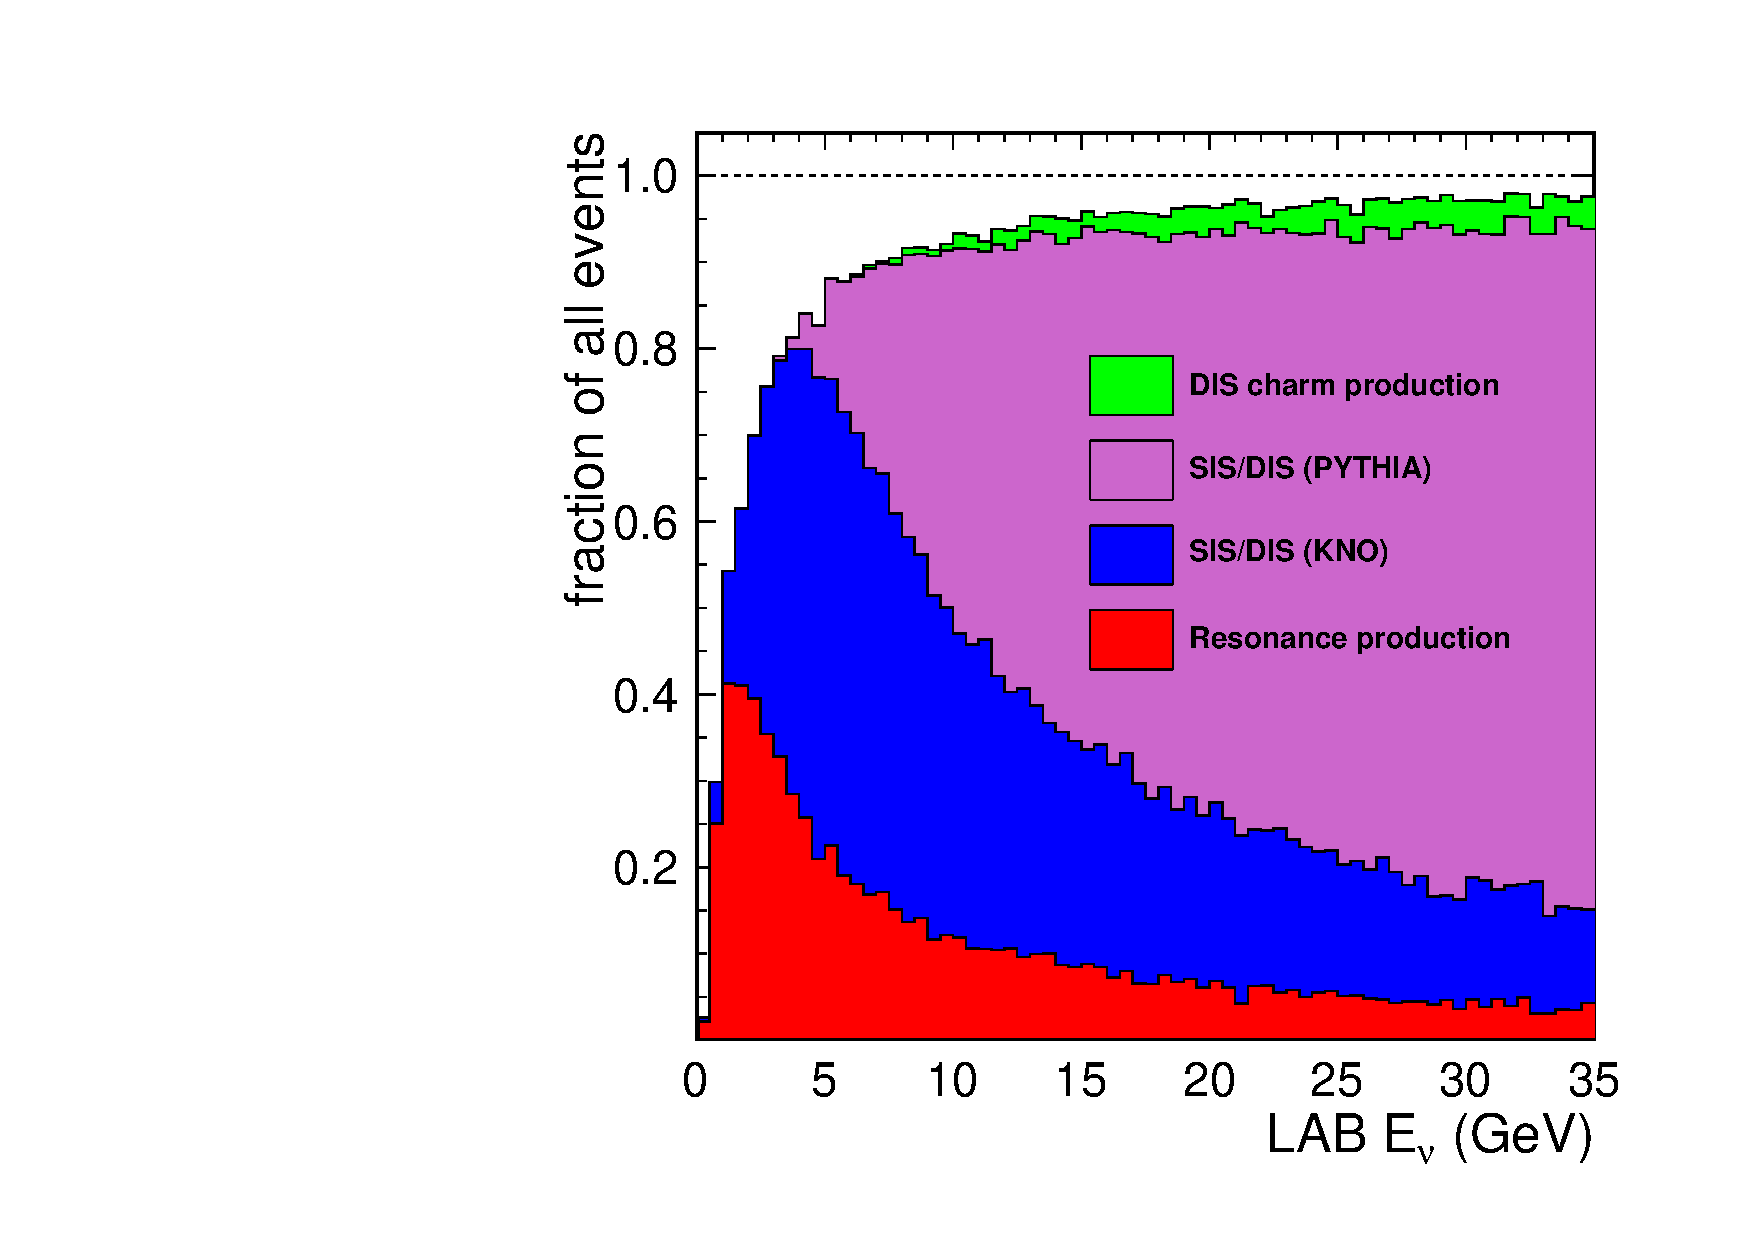
\includegraphics[width=0.98\textwidth]{./images/nuint/dis/hadrofracE.pdf}
  \end{column}
  \begin{column}{0.50\textwidth}
     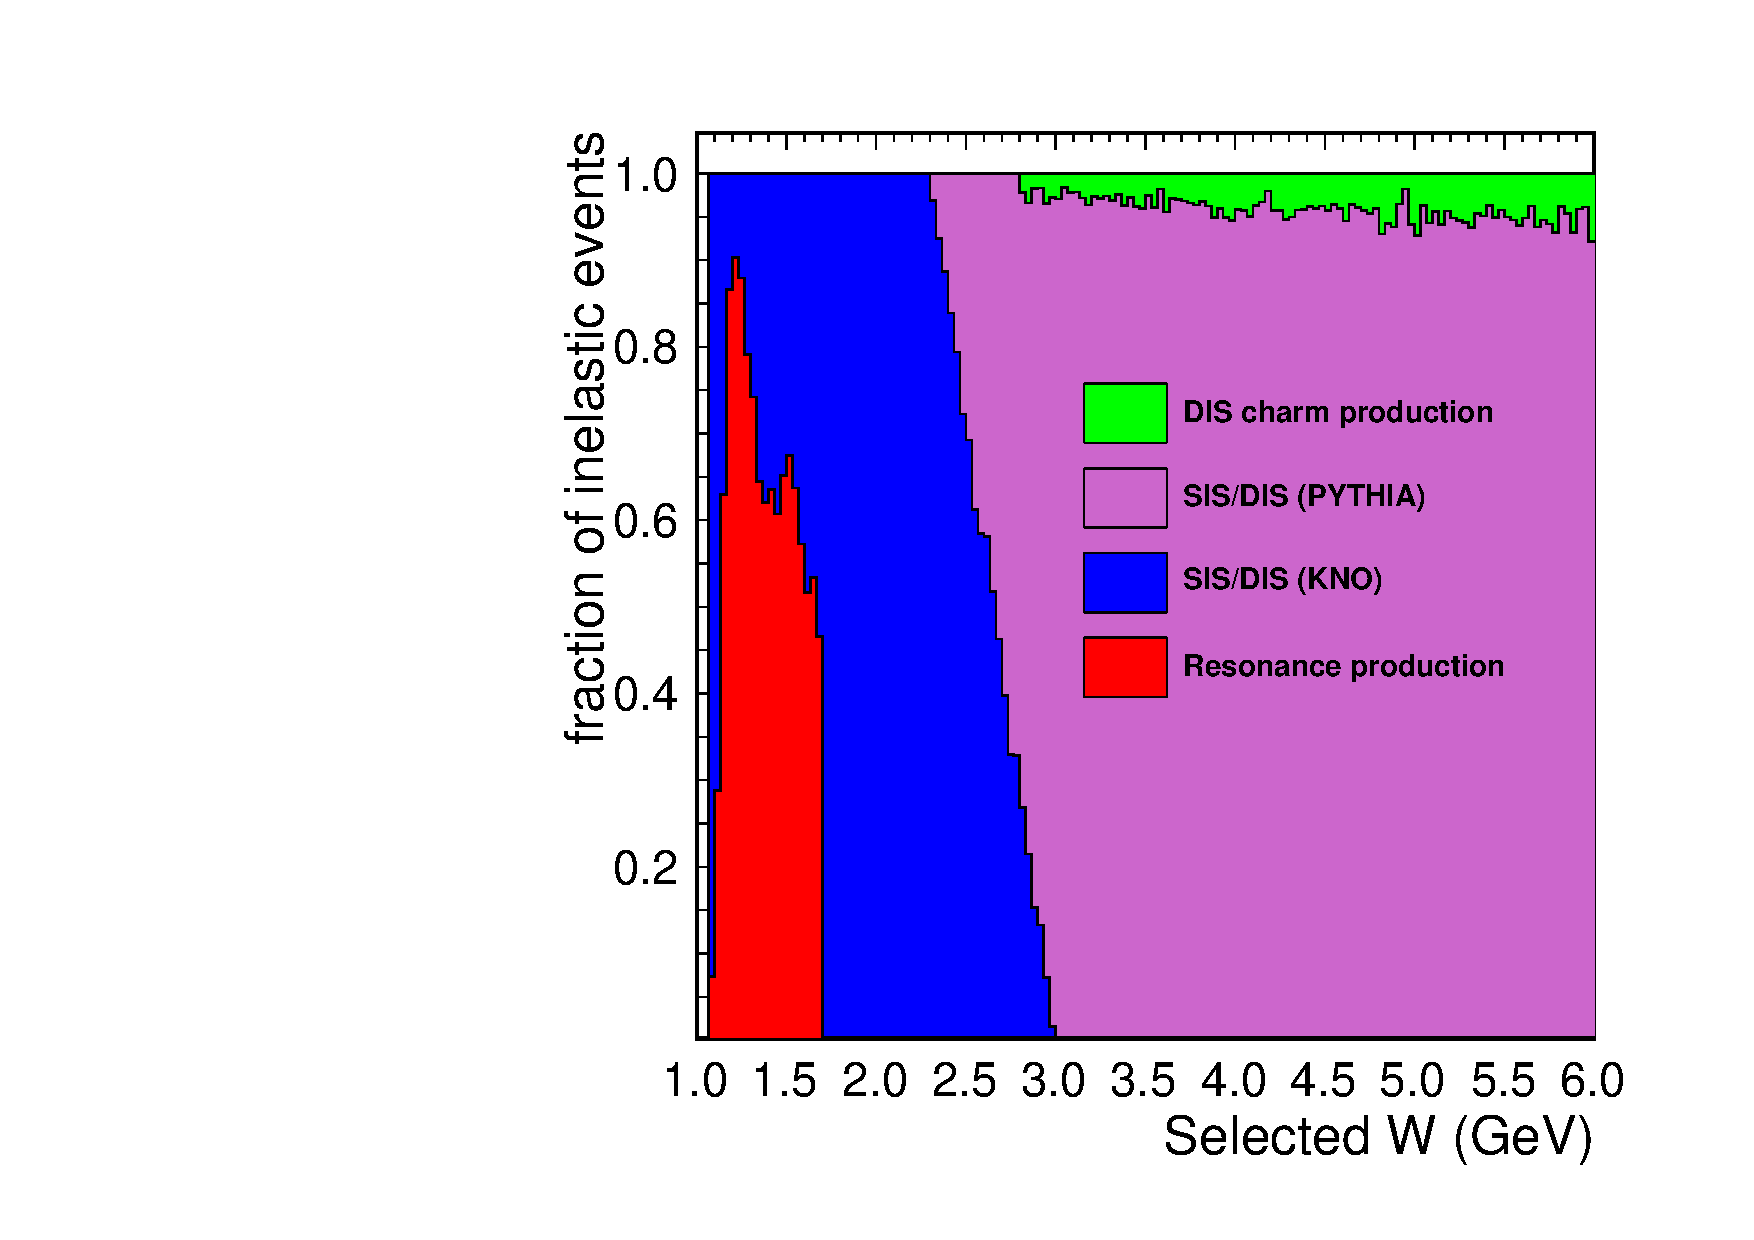
\includegraphics[width=0.98\textwidth]{./images/nuint/dis/hadrofracW.pdf}
  \end{column}
\end{columns}
{\scriptsize
 Very important modelling aspect. The shower shape, energy profile and particle
 content important for energy reconstruction and event identification.
}
\end{frame}


\begin{frame}{Hadronization for Shallow and Deep Inelastic Scattering}

The basic picture of hadronization:\\
\begin{center}
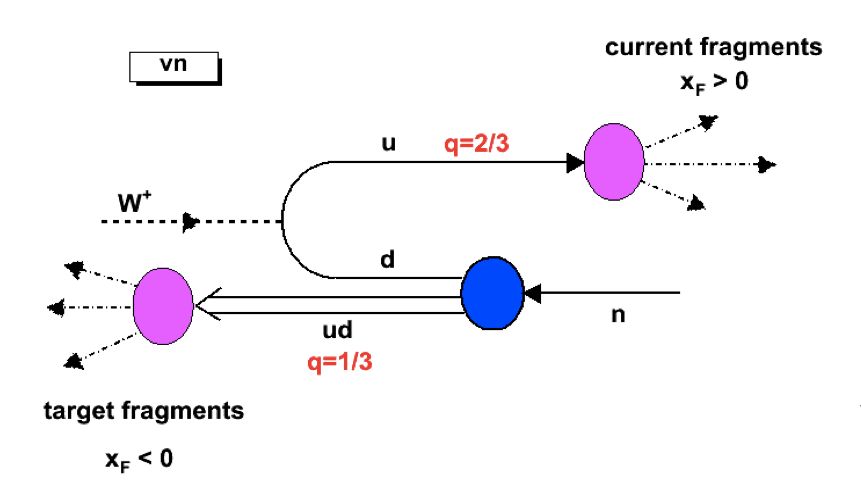
\includegraphics[width=270px]{./images/nuint/dis/fragments.png}
\end{center}
\end{frame}


\begin{frame}{PYTHIA}

\begin{itemize}
\item LUND string fragmentation model
\item Uses the assumption of linear confinement as a starting point.
\item As partons move apart, their colour flux tube gets stretched.
\item Stored potential energy increases linearly with distance of colour charges.
\item You can think of the "string" as the axis of the flux tube.
\item The string constant is $\sim$ 1 GeV/fm.
\item As the potential energy increases, the string may break producing a $q\bar{q}$ pair.
\item String breaks causally disconnected; simulated in a convenient order.
\item A break typically creates a meson.
\item Baryons also produced; A string can break by anti{\bf}diquark-{\bf}diquark production, or baryons can be produced using a `popcorn' model.
\item With every break, a produced hadron takes away a fraction of the available energy/momentum.
\item Continuing till some cut-off point.
\end{itemize}
\end{frame}


\begin{frame}{PYTHIA tuning}

\begin{table}[ht]
\centering
\begin{tabular}{| c || c | c | c |}
\hline
                                              &  PYTHIA    & NUX   & GENIE \\
                                              &  default   & 2001  & 2010 re-tune \\
\hline
  $s\bar{s}$ production suppression           &    0.30    & 0.21        & 0.30      \\
  $<p_{T}^{2}>$ ($GeV^{2}$)                   &    0.36    & 0.44        & 0.44      \\
  Non-gaussian $p_{T}$ tail parameterization  &    0.01    & 0.01        & 0.01      \\
  Fragmentation cut-off energy (GeV)          &    0.80    & 0.20        & 0.20      \\
\hline
\end{tabular}
\end{table}
\end{frame}


\begin{frame}{Data on neutrino-induced hadron shower characteristics}

Several pieces of data exist.\\
\vspace{0.3cm}
\begin{itemize}
  \item Average charged and neutral particle multiplicities
  \item Forward and backward hemisphere average multiplicities
  \item Forward and backward hemisphere charge distributions
  \item Multiplcity correlations (e.g. charged hadrons - $\pi^{0}$)
  \item Multiplicity distributions
  \item Fragmentation functions (z distributions)
  \item $x_{F}$ distributions
  \item $p_{T}^{2}$ distributions
  \item $x_{F}$ - $p_{T}^{2}$ distributions
\end{itemize}

However, coverage of the low - W range (W $<$ 4-5 GeV is poor)

\end{frame}


\begin{frame}{Effective KNO-based hadronization model}

\begin{itemize}
 \item An {\bf effective KNO-based hadronization model was built} 
       (T.Yang, H.Gallagher, P.Kehayias, CA - circa 2007) for low W and was "integrated" with PYTHIA to cover the 
       full kinematic space (AGKY model, Eur.Phys.J.C63:1-10,2009)
 \item The model was {\bf anchored on several pieces of bubble chamber data and captures several observations 
       on the characteristics of neutrino-induced hadron showers} (for an excellent description, see Norbert Schmitz,
       Adv.Ser.Direct.High Energy Phys. 2 (1988) 3-56)
 \item A similar, KNO-inspired model pre-existed in neugen3. 
       Several model improvements were installed in 2007-2008, particularly in the algorithm for generating the hadron momenta,
       to simulate the forward/backward asymmetry and $p_{T}$ squeezing seen in data, but not described by earlier versions of the model.
 \item Extensive data/MC comparisons were performed (T.Yang).
 \item Several caveats were recognized over time; few improvements were made (e.g strange baryon production by K.Hoffmann, H.Gallagher)
\end{itemize}
\end{frame}



\begin{frame}{Effective KNO-based hadronization model}

For a given event (given neutrino and hit nucleon, given interaction type (CC/NC) and hadronic invariant mass W) 
the hadronization model needs to generate answers to the following questions:\\
\vspace{0.2cm}
\begin{itemize}
 \item How many hadrons are produced?
 \item What are the hadron IDs?
 \item What are the hadron 4-momenta?
\end{itemize}
\vspace{0.2cm}
At every point, we make decisions that depend on data (with errors) or on assumptions 
(usually well motivated, but simplified).\\
Several sources of systematic uncertainty.
\end{frame}




\begin{frame}{KNO-based model: How many hadrons are produced?}

First, we answer that question "on average".
The model uses measured average charged hadron multiplicities $<n_{ch}>$ which are described well by:\\
\[
  <n_{ch}> = a + b \cdot log(W^{2})
\]
The values of a,b used are:\\
\begin{table}[ht]
\centering
\begin{tabular}{| c || c | c | c | c |}
\hline
           &    ${\nu}p$         & ${\nu}n$          &  ${\bar{\nu}}p$  & ${\bar{\nu}}n$ \\
\hline
  a        &    0.40             & -0.20             &  0.02            & 0.80  \\
  b        &    1.42             & -1.42             &  1.28            & 0.95  \\
\hline
\end{tabular}
\end{table}
The average neutral hadron multiplicity was measured to be about $\frac{1}{2}$ of the
average charged hadron multiplicity. This allows us to calculate the average total
hadron multiplicity $<n_{tot}>$ as:\\
\[
  <n_{tot}> = 1.5 <n_{ch}>
\]
\end{frame}



\begin{frame}{Average charged multiplicities}
\begin{center}
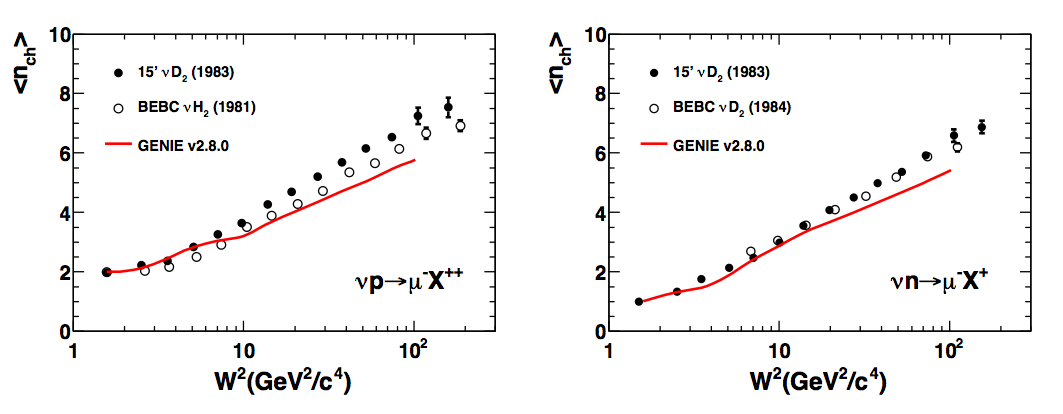
\includegraphics[width=280px]{./images/nuint/dis/avgnch_vs_W2.png}\\
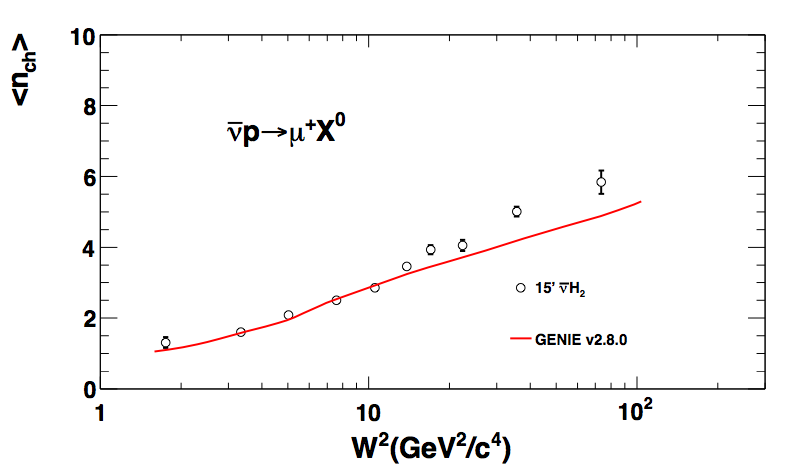
\includegraphics[width=190px]{./images/nuint/dis/avgnch_vs_W2_nubar.png}\\
\end{center}
\end{frame}

\begin{frame}{Average neutral multiplicities}
\begin{center}
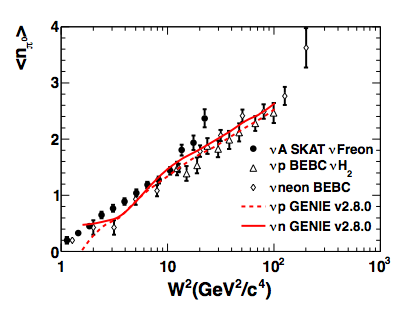
\includegraphics[width=180px]{./images/nuint/dis/avgnpi0_vs_W2.png}
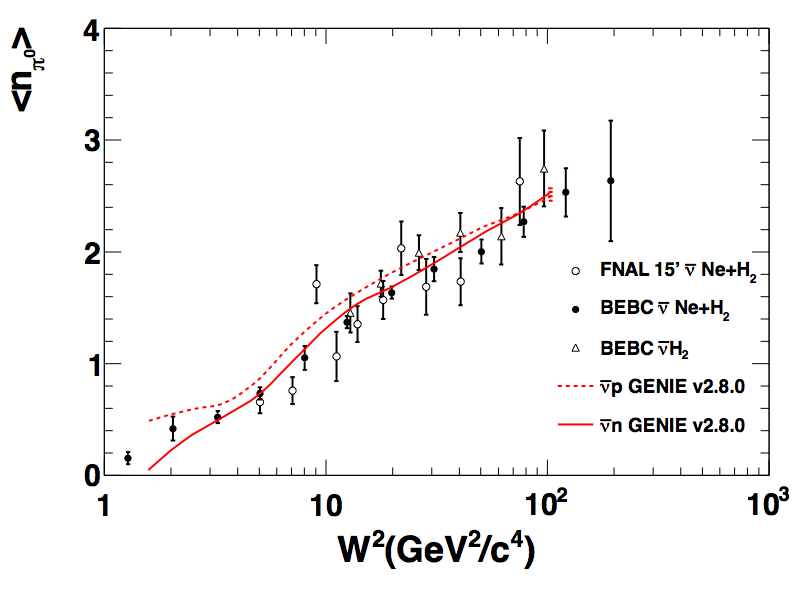
\includegraphics[width=180px]{./images/nuint/dis/avgnpi0_vs_W2_nubar.png}\\
\end{center}
\end{frame}


\begin{frame}{KNO-based model: How many hadrons are produced?}
Based on the calculated average total hadron multiplity $<n_{tot}>$, we can draw actual total multiplicities $n_{tot}$ on an event-by-event basis.\\
The particles are not "independently" produced and the actual multiplicity is not Poisson-distributed.
Multiplicities are generated based on the KNO-scaling law (i.e. the observation that $<n>P(n) = f(n/<n>)$ is independent of W).\\
The function $f(z=n/<n>)$ is parameterized using the Levy function with parameter c:
\[
L(z;c) = \frac{2e^{c}c^{cz+1}}{\Gamma(cz+1)}
\]
The following parameters c were determined by a fit to data (T.Yang):\\
\begin{table}[ht]
\centering
\begin{tabular}{| c | c | c | c |}
\hline
  ${\nu}p$         & ${\nu}n$          &  ${\bar{\nu}}p$  & ${\bar{\nu}}n$ \\
\hline
  7.93 $\pm$ 0.34  & 5.22 $\pm$ 0.15   &  as ${\nu}n$     & as ${\nu}p$    \\
\hline
\end{tabular}
\end{table}
Caveat: $<n_{ch}>P(n_{ch}) = f(n_{ch}/<n_{ch}>)$ is independent of W. Assume this applies for the total multiplicity too.
\end{frame}

\begin{frame}{KNO scaling}
\begin{center}
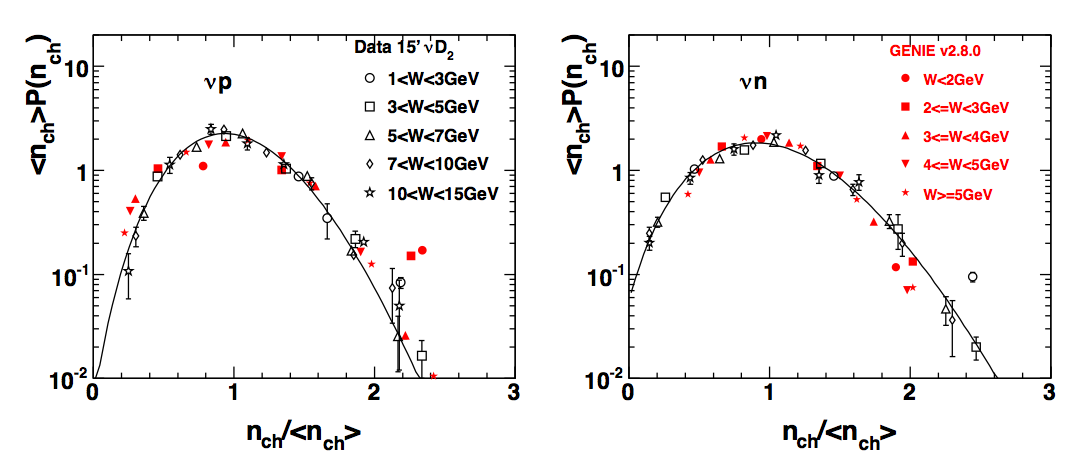
\includegraphics[width=330px]{./images/nuint/dis/kno.png}
\end{center}
\end{frame}

\begin{frame}{Multiplicity dispersion}
\begin{center}
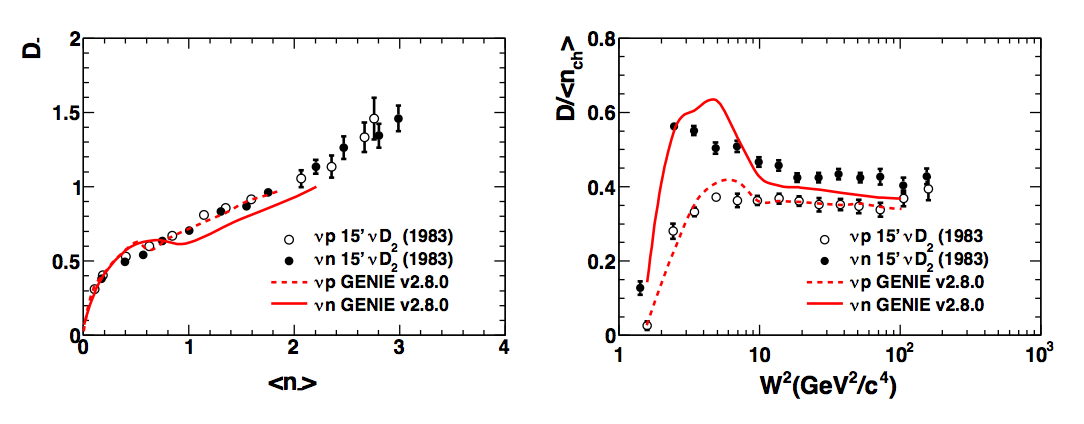
\includegraphics[width=280px]{./images/nuint/dis/dispersion_ch.png}\\
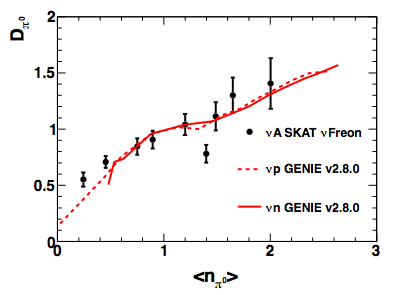
\includegraphics[width=170px]{./images/nuint/dis/dispersion_pi0.png}\\
\end{center}
\end{frame}

\begin{frame}{Topological cross-sections}
\begin{center}
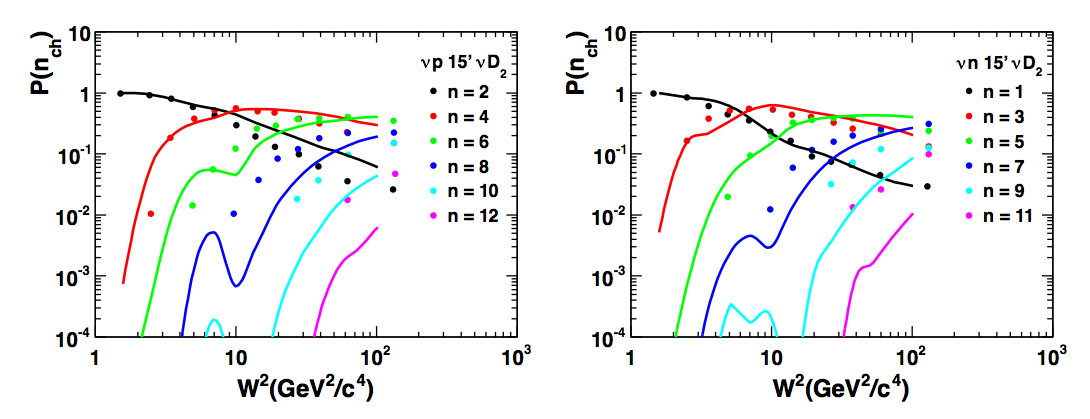
\includegraphics[width=280px]{./images/nuint/dis/topological_xsecs.png}\\
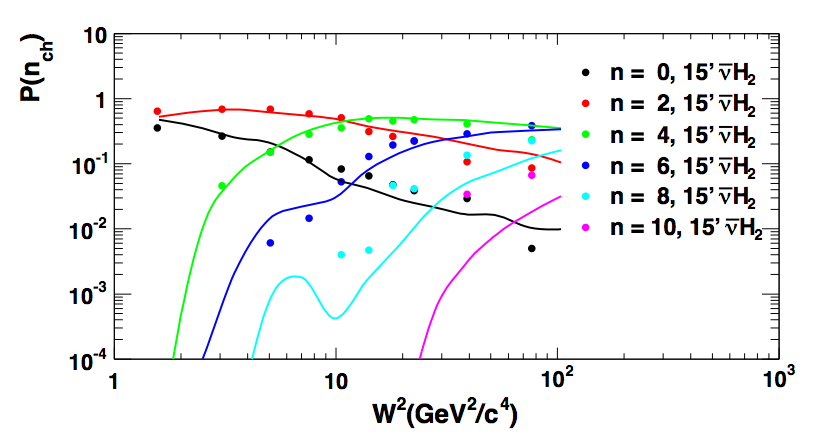
\includegraphics[width=210px]{./images/nuint/dis/topological_xsecs_nubar.png}\\
\end{center}
\end{frame}



\begin{frame}{KNO-based model: Selecting the particle IDs}

Once we have decided the actual particle multiplicity, we need to decide the particle codes.
One of the the particles would be a baryon.\\
We decide between a p or n, with the following probabilities\\

\begin{table}[ht]
\centering
\begin{tabular}{| c || c | c | c | c |}
\hline
 $n_{tot}$ &    ${\nu}p$         & ${\nu}n$          &  ${\bar{\nu}}p$  & ${\bar{\nu}}n$ \\
\hline
  2        &    1.00             & 0.33              &  0.67            & 0.    \\
  $>$2     &    0.67             & 0.50              &  0.50            & 0.33  \\
\hline
\end{tabular}
\end{table}

Subsequently, one of those will be converted to a strange baryon (for $\nu$ interactions: p $\rightarrow \Sigma^{+}$ and n $\rightarrow \Lambda$;
for $\bar{\nu}$ interactions: p $\rightarrow \Lambda$ and n $\rightarrow \Sigma^{-}$)\\

The probability for generating a strange baryon is given by:\\
\[
<n_{hyperon}> = a_{hyperon} + b_{hyperon} \cdot log(W^{2})
\]
where
\begin{table}[ht]
\centering
\begin{tabular}{| c || c | c | c | c |}
\hline
                     &    ${\nu}p$         & ${\nu}n$          &  ${\bar{\nu}}p$  & ${\bar{\nu}}n$ \\
\hline
 $a_{hyperon}$       &    0.022            &  0.022            &  0.022           & 0.022  \\
 $b_{hyperon}$       &    0.042            &  0.042            &  0.042           & 0.042  \\
\hline
\end{tabular}
\end{table}

\end{frame}


\begin{frame}{KNO-based model: Selecting the particle IDs}

Once a baryon (p, n or hyperon) were selected, the remaining $n_{tot}$-1 particles would be mesons.\\
\vspace{0.1cm}
If a strange baryon was added, we add a strange meson to conserve strangeness (no ${\Delta}$S=1 
production in hadronization; this is added separately).\\
\vspace{0.1cm}
Then, keep on adding $\pi^{+}$ or $\pi^{-}$ till charge is balanced.\\
\vspace{0.1cm}
Then add particles in pairs till all $n_{tot}$ particle codes have been assigned.\\
Particle pairs are added with the following probabilities:\\
\begin{table}[ht]
\centering
\begin{tabular}{| c | c | c | c |}
\hline
       $\pi^{0}\pi^{0}$   & $\pi^{+}\pi^{-}$     &  $K^{0}\bar{K^{0}}$  & $K^{+}K^{-}$ \\
\hline
       0.3133             &  0.6267              &  0.03                & 0.03  \\
\hline
\end{tabular}
\end{table}

\end{frame}




\begin{frame}{KNO-based model: Generating particle momenta}

\begin{columns}[T]
  \begin{column}{0.40\textwidth}
     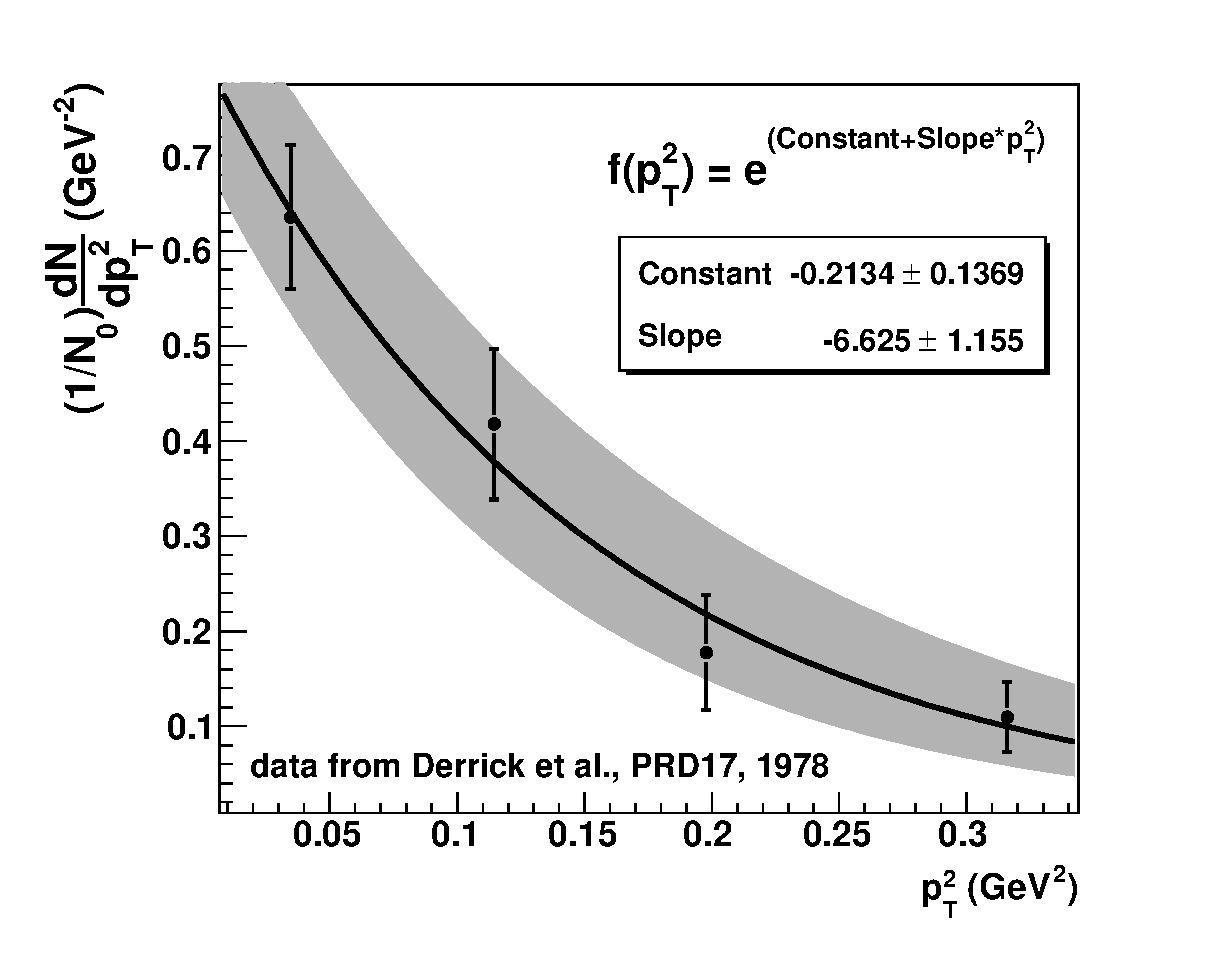
\includegraphics[width=0.93\textwidth]{./images/nuint/dis/nucpT2pdf.eps}\\
     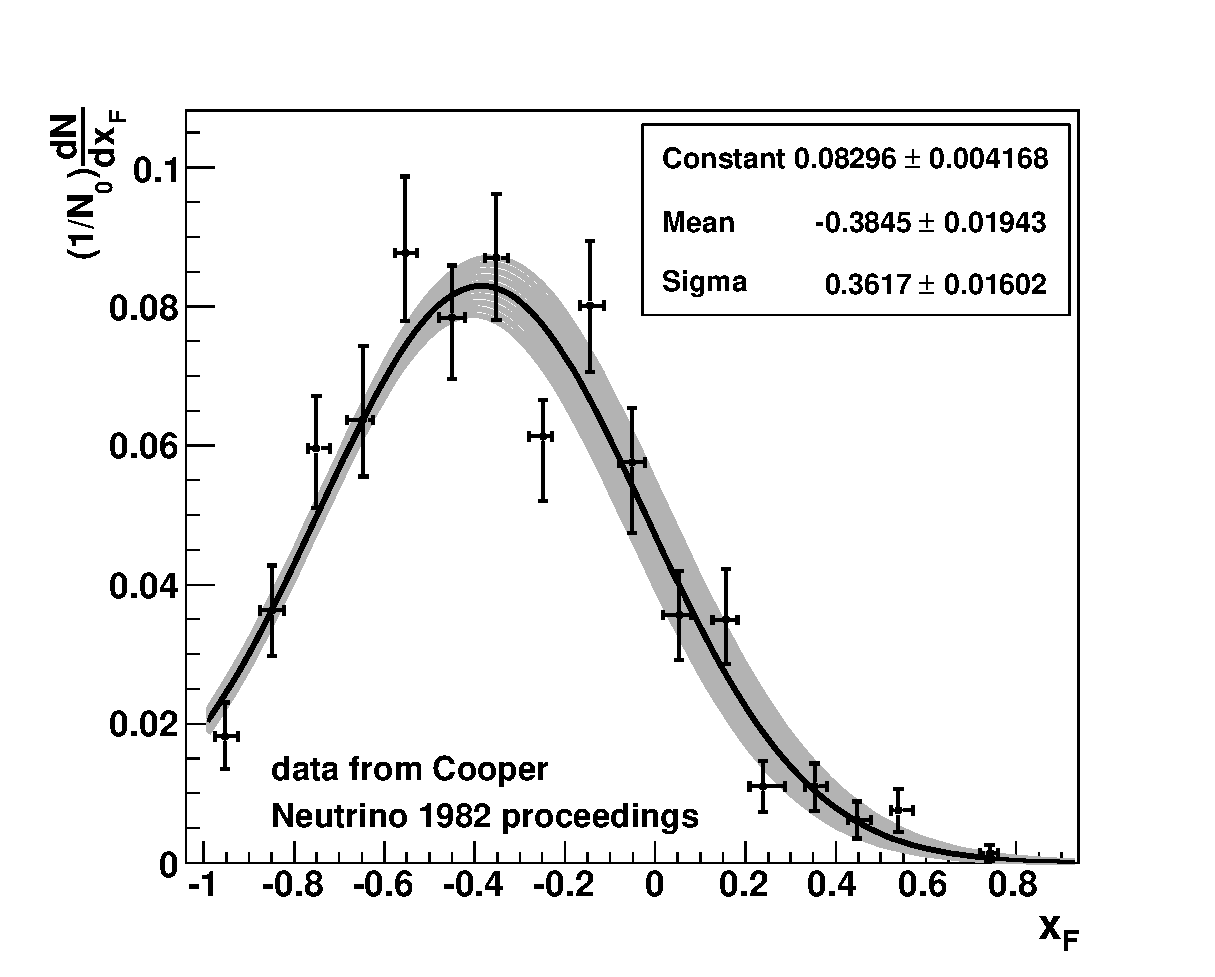
\includegraphics[width=0.93\textwidth]{./images/nuint/dis/nucxFpdf.eps}
  \end{column}
  \begin{column}{0.60\textwidth}
      Baryon $p_{T}$ and $x_{F}$ selected using a measured distribution as p.d.f.\\
      This has important consequences for the shower shape.\\
      Since the heavy baryon is generated predominantly backwards, more light mesons
      are produced in the forward hemisphere.\\
      The used empirical distribution was not published.\\
      There is evidence that the shower shape should have been more fwd/bkw-symmetric at lower W.
      There is a systematic handle to shift the used $x_{F}$ p.d.f. for low multiplicity hadronic
      states important in T2K.
  \end{column}
\end{columns}
\end{frame}


\begin{frame}{KNO-based model: Generating particle momenta}

\begin{columns}[T]
  \begin{column}{0.60\textwidth}
    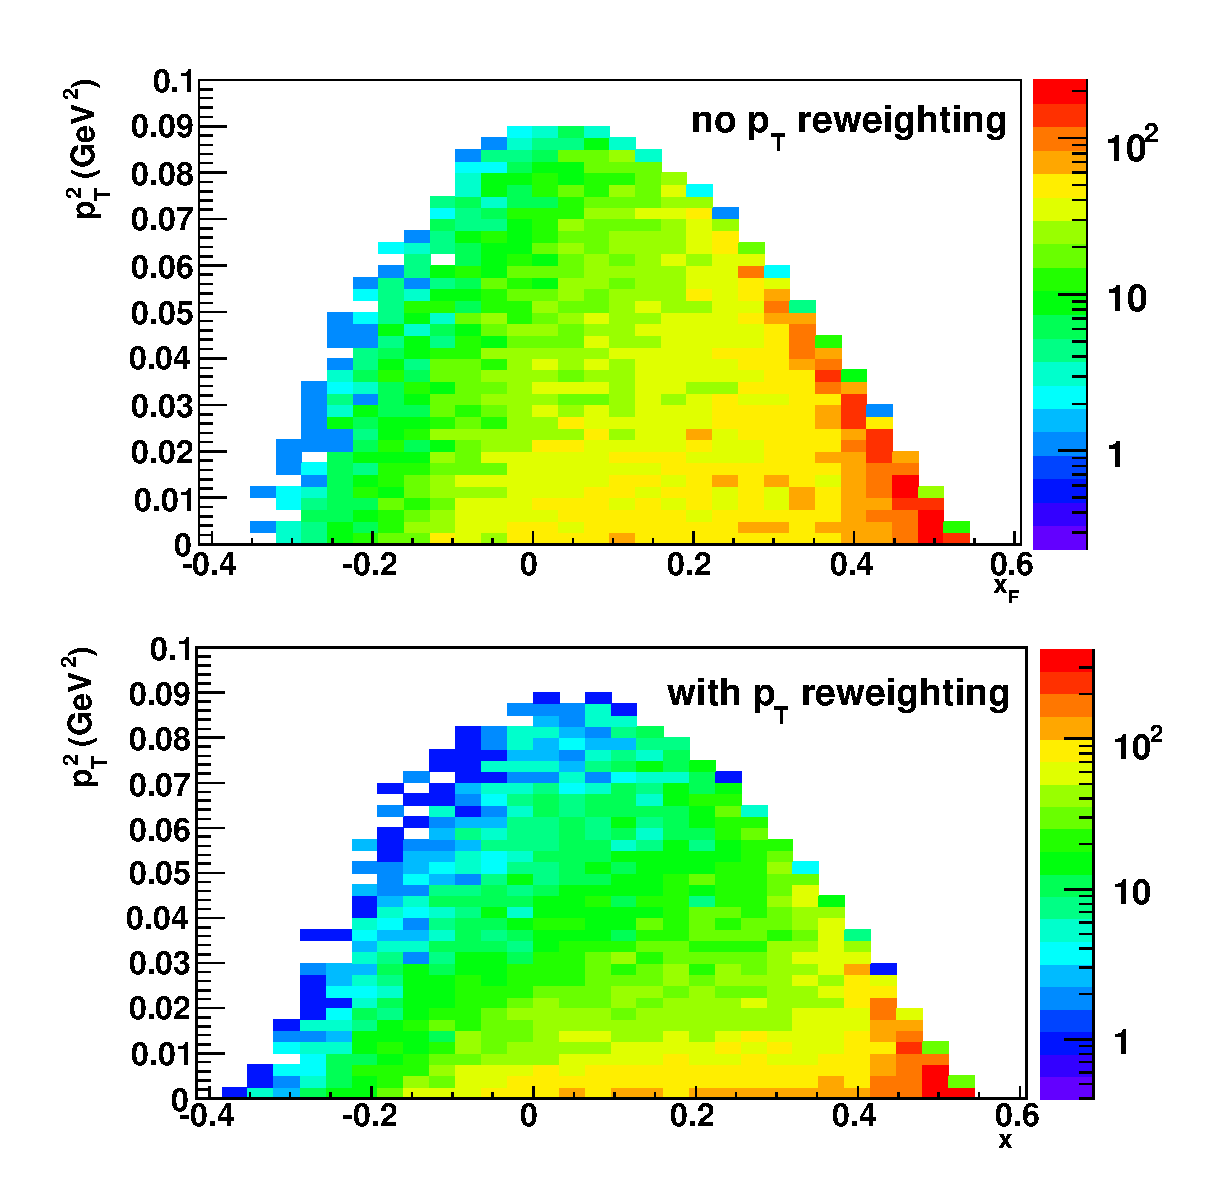
\includegraphics[width=200px]{./images/nuint/dis/pT2ReweightExample.eps}\\
  \end{column}
  \begin{column}{0.40\textwidth}
     The rest of the system is generated via a phase space decay.\\
     Using the idea of Clegg and Donnachie
     (“Description of Jet Structure by pt-limited Phase Space”, Z. Phys. C 13: 71 (1982))
     to squeeze the phase space by decreasing the likelihood of higher $p_{T}$ values.\\
     A factor of $e^{-A \cdot p^{i}_{T}}$ (A = 3.5 $GeV^{-1}$) 
     is included for each hadron in the phase space decay weight.
  \end{column}
\end{columns}
\end{frame}


\begin{frame}{Average charged multiplicities in fwd/bkw hemisphere}

\begin{center}
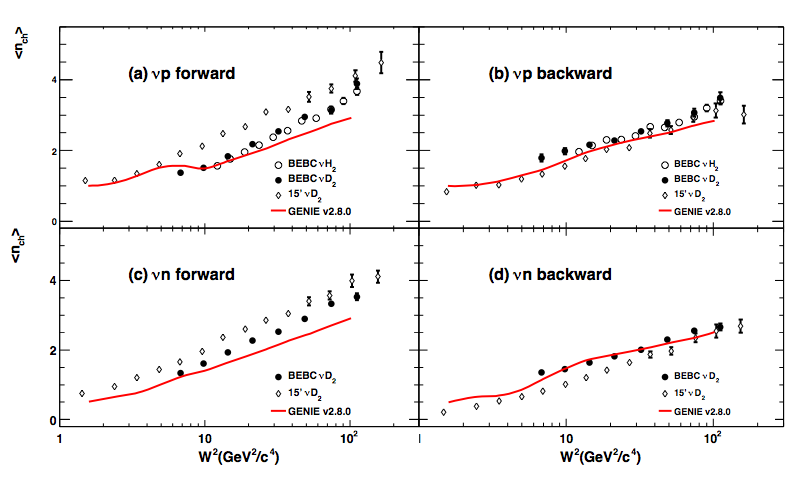
\includegraphics[width=280px]{./images/nuint/dis/avgnch_vs_W2_FB.png}\\
\end{center}
\end{frame}


\begin{frame}{$x_{F}$ and z distributions}

\begin{center}
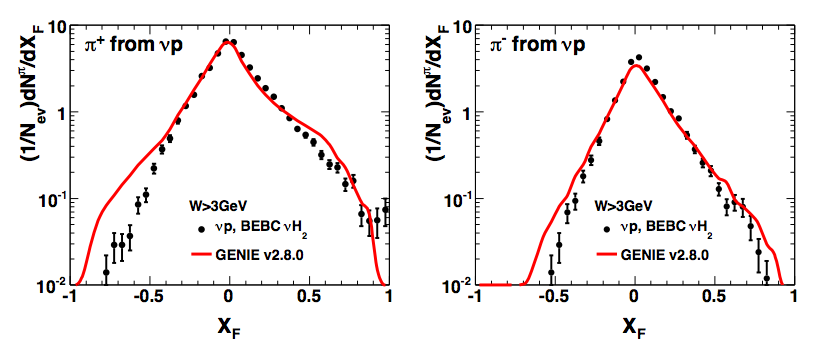
\includegraphics[width=250px]{./images/nuint/dis/xF_distribution.png}\\
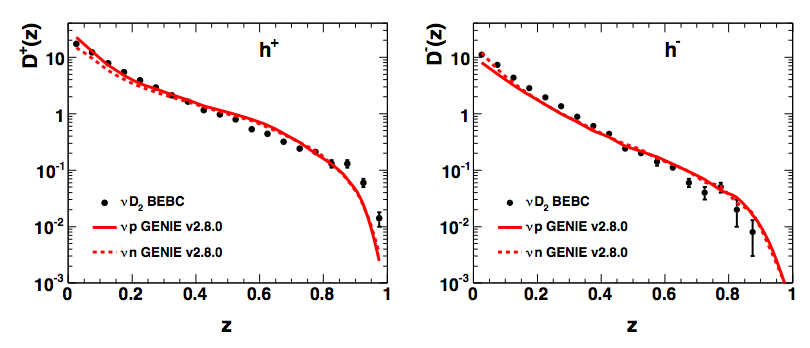
\includegraphics[width=250px]{./images/nuint/dis/z_distribution.png}\\
\end{center}
\end{frame}

\begin{frame}{$p_{T}$ distributions}

\begin{center}
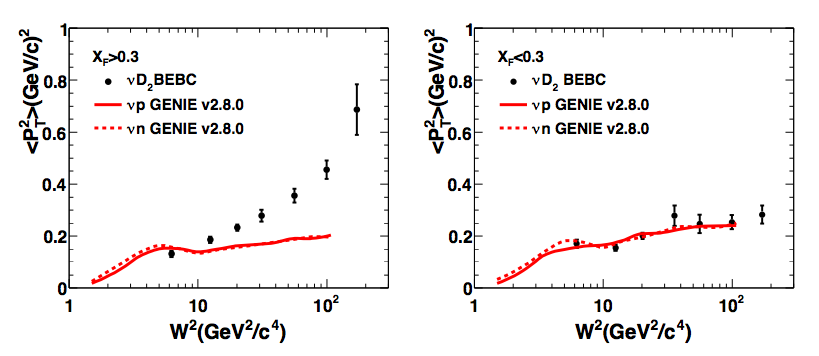
\includegraphics[width=240px]{./images/nuint/dis/pT2_distribution_1.png}\\
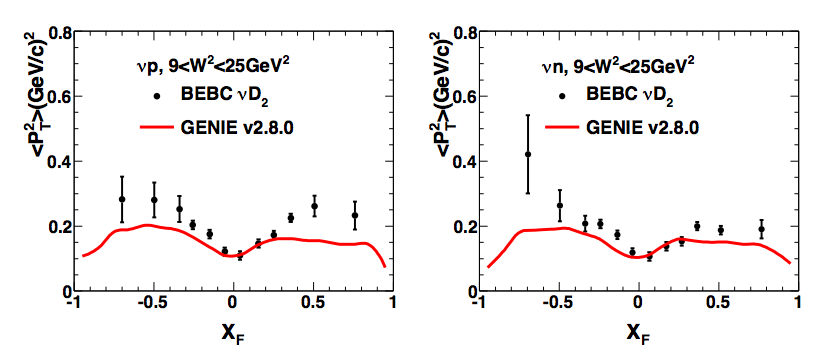
\includegraphics[width=240px]{./images/nuint/dis/pT2_distribution_2.png}\\
\end{center}
\end{frame}


\begin{frame}{PYTHIA and KNO reweighting}

PYTHIA a black box. There are some tuning handles, but no event-by-event reweighting functions.\\
\vspace{0.3cm}
The KNO-based model is not a black box, but no full, exact reweighting exists either.
This is because it is hard.
\begin{itemize}
 {\small
  \item Some, brute-force $x_{F}$ and $p_{T}$ reweighting capability for 2-hadron final states was installed for T2K.
  \item Some ongoing work by N.Mayer and A.Norrick together with GENIE authors.
  \item Some additional reweighting capability in private versions of the code, but not complete.
 }
\end{itemize}

For the initial VALOR fits, we will construct the hadronization systematic covariance matrix without reweighting (see next).\\

{\bf But first, a study is needed to establish a reasonable range of all input parameters, using the data/MC comparisons shown previously}

\end{frame}


\begin{frame}{DIS charm production}

For DIS charm production, there is a separate hadronization model.\\

\begin{columns}[T]
  \begin{column}{0.50\textwidth}
     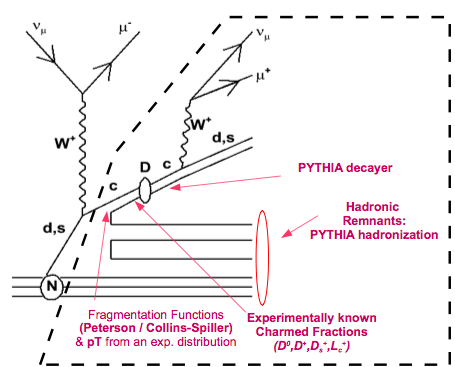
\includegraphics[width=0.98\textwidth]{./images/nuint/dis/charm_hadro.png}
  \end{column}
  \begin{column}{0.50\textwidth}
     \begin{itemize}
     {\small
       \item Generate the charm hadron energy using the Peterson or Collins-Spiller fragmentation functions
       \item Generate the charm hadron ID ($D^{0}$, $D^{\pm}$, $D_{s}^{\pm}$,$\Lambda_{c}^{+}$) using experimentally measured charm fractions
       \item Use PYTHIA for the remnant hadronic system
     }
     \end{itemize}
  \end{column}
\end{columns}
\vspace{0.2cm}
To date, there is no reweighting model for charm production.\\
The fragmentation function and charm fractions are the obvious candidates to be tweaked (along with Vcs, Vcd, $m_{charm}$ in the cross-section model).\\
\end{frame}


\begin{frame}{Resonance Decays}

The pion angular distribution $W_{\pi}(cos\theta)$ in 
$\Delta \rightarrow N \pi$ decay can be expressed as\\
\[
W_{\pi}(cos\theta) = 1 - p(\frac{3}{2}) P_{2}(cos\theta) + p(\frac{1}{2}) P_{2}(cos\theta)
\]
where $\theta$ is the pion production angle in the $\Delta$ 
center of mass frame with respect to the $\Delta$ angular momentum quantization axis, 
$P_{2}$ is the 2nd order Legendre polynomial 
and $p(\frac{3}{2})$, $p(\frac{1}{2})$ are coefficients.\\
\vspace{0.2cm}
The Rein-Sehgal (RS) model predicts $p(\frac{3}{2})$ = 0.75 and $p(\frac{1}{2})$ = 0.25.\\
\vspace{0.2cm}
For simplicity, GENIE decays baryon resonances isotropically during event generation. 
Isotropy requires $p(\frac{3}{2})$ = $p(\frac{1}{2})$ = 0.5.\\
\vspace{0.2cm}
The difference between the two can be taken as a "systematic".
\end{frame}


\begin{frame}{Resonance Decays}

\begin{columns}[T]
  \begin{column}{0.50\textwidth}
    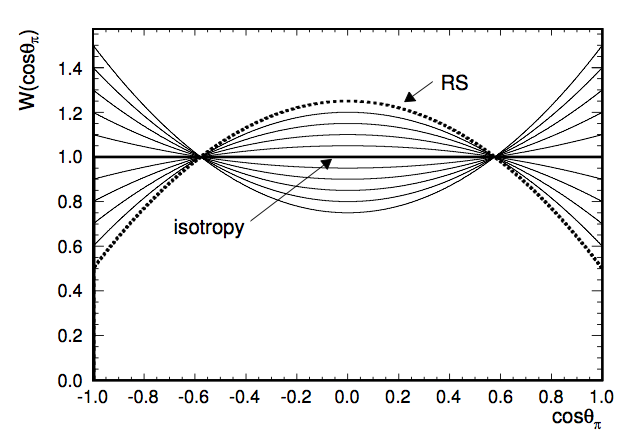
\includegraphics[width=170px]{./images/nuint/dis/res_dec_rewght.png}
  \end{column}
  \begin{column}{0.50\textwidth}
   {\small
     A systematic handle is already included in GENIE to tweak the angular distributions
     of resonance decay products.\\
     Currently, tweaking only the decay of the P33(1232) $\Delta$ resonance to $p+\pi^{+}$
     (as this is what mattered most for T2K) but could be expanded to other resonances and
     decay channels.\\
   }
  \end{column}
\end{columns}
\vspace{0.2cm}
The probability that the resonance was created in the first place and
whether it re-interacted (eg via  $\Delta+N \rightarrow N+N$) are also important
sources of systematics, but not in the domain of the "hadronization model".
\end{frame}


\begin{frame}{In-medium effects to hadronization}

In-medium effects to handronization are included using a single formation time of 0.342 fm/c\\

A reweighting handle exists in GENIE, but effect not fully reweightable.\\

\begin{itemize}
\item No "coherence length" in default simulation (but implemented by George in March)
  \begin{itemize}
    \item Needed???
    \item Need special samples to evaluate uncertainty
  \end{itemize}
\item In default simulation, formation zone applied only in DIS events,
  \begin{itemize}
    \item Needed for other modes???
    \item Need special samples to evaluate uncertainty on RES events
  \end{itemize}
\end{itemize}

Also, again, more data/MC studies are needed. Some of these were started by Athans.

\end{frame}


\begin{frame}{In-medium effects to hadronization}
\begin{center}
  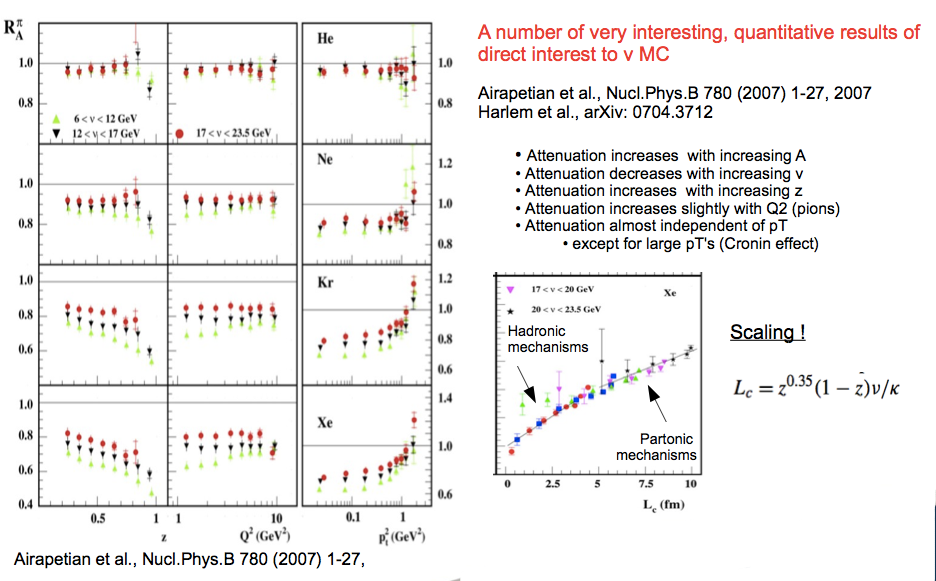
\includegraphics[width=0.98\textwidth]{./images/nuint/dis/hermes_slide.png}
\end{center}
\end{frame}


